\chapter{Introduction}
\label{ch:intro}
Electricity is used every day by the majority of Americans, but is largely consumed without thought.  Often people notice electricity, and their consumption of it, when they no longer have access to it; perhaps there is a brief power surge, or even a total blackout, which reminds us that our ability to see in the dark is a fragile luxury, that we often take for granted.  Blackouts, or cascading failures, are ubiquitous in power systems, because we use the power system as cost-effectively as possible \cite{na_cf_stats}.  The study of cascading failure dynamics in power systems started at the turn of the century, and draws researchers from a multitude of backgrounds such as electrical engineering, network science, and even cyber-security.  The ultimate goal for many researchers is to predict and/or prevent blackouts as a way to ensure reliable access to power.  However, as I hope becomes clear throughout this paper, I'll show that a better understanding of the underlying mechanisms and dynamics of cascading failures is not only an interesting and challenging problem, but also necessary for any hope in controlling them.



Any research regarding modern power systems must account for the changes occurring due to the reconfiguration of our power sources.  We are no longer able to ignore the fact that there is a demonstrable need to replace fuel sources that contribute large amounts of greenhouse gas emissions. According to the Environmental Protection Agency, electricity is one of the largest contributors of greenhouse gases in the US, only slightly below transportation \cite{greenhouse_gas}.  Up until very recently, the majority of these emissions were due to a significant use of coal as a fuel source for electricity, seen on the right side of Figure \ref{fig:ghg}.  However, based on the lowering price of natural gas and renewable resources such as wind and solar photovoltaics (PV), it is expected that renewable resources will contribute at least as much as coal by the year 2050\footnote{Note: These projections do not consider the Clean Power Plan implemented in 2014.} (see left panel of Figure \ref{fig:ghg}) \cite{eia_eo}.  If protecting the environment is not enough reason, consider that the cost of For these reasons, it has become more and more important to consider how renewable resources like wind and solar PV alter how our electricity infrastructure functions.

\begin{figure}
\centering
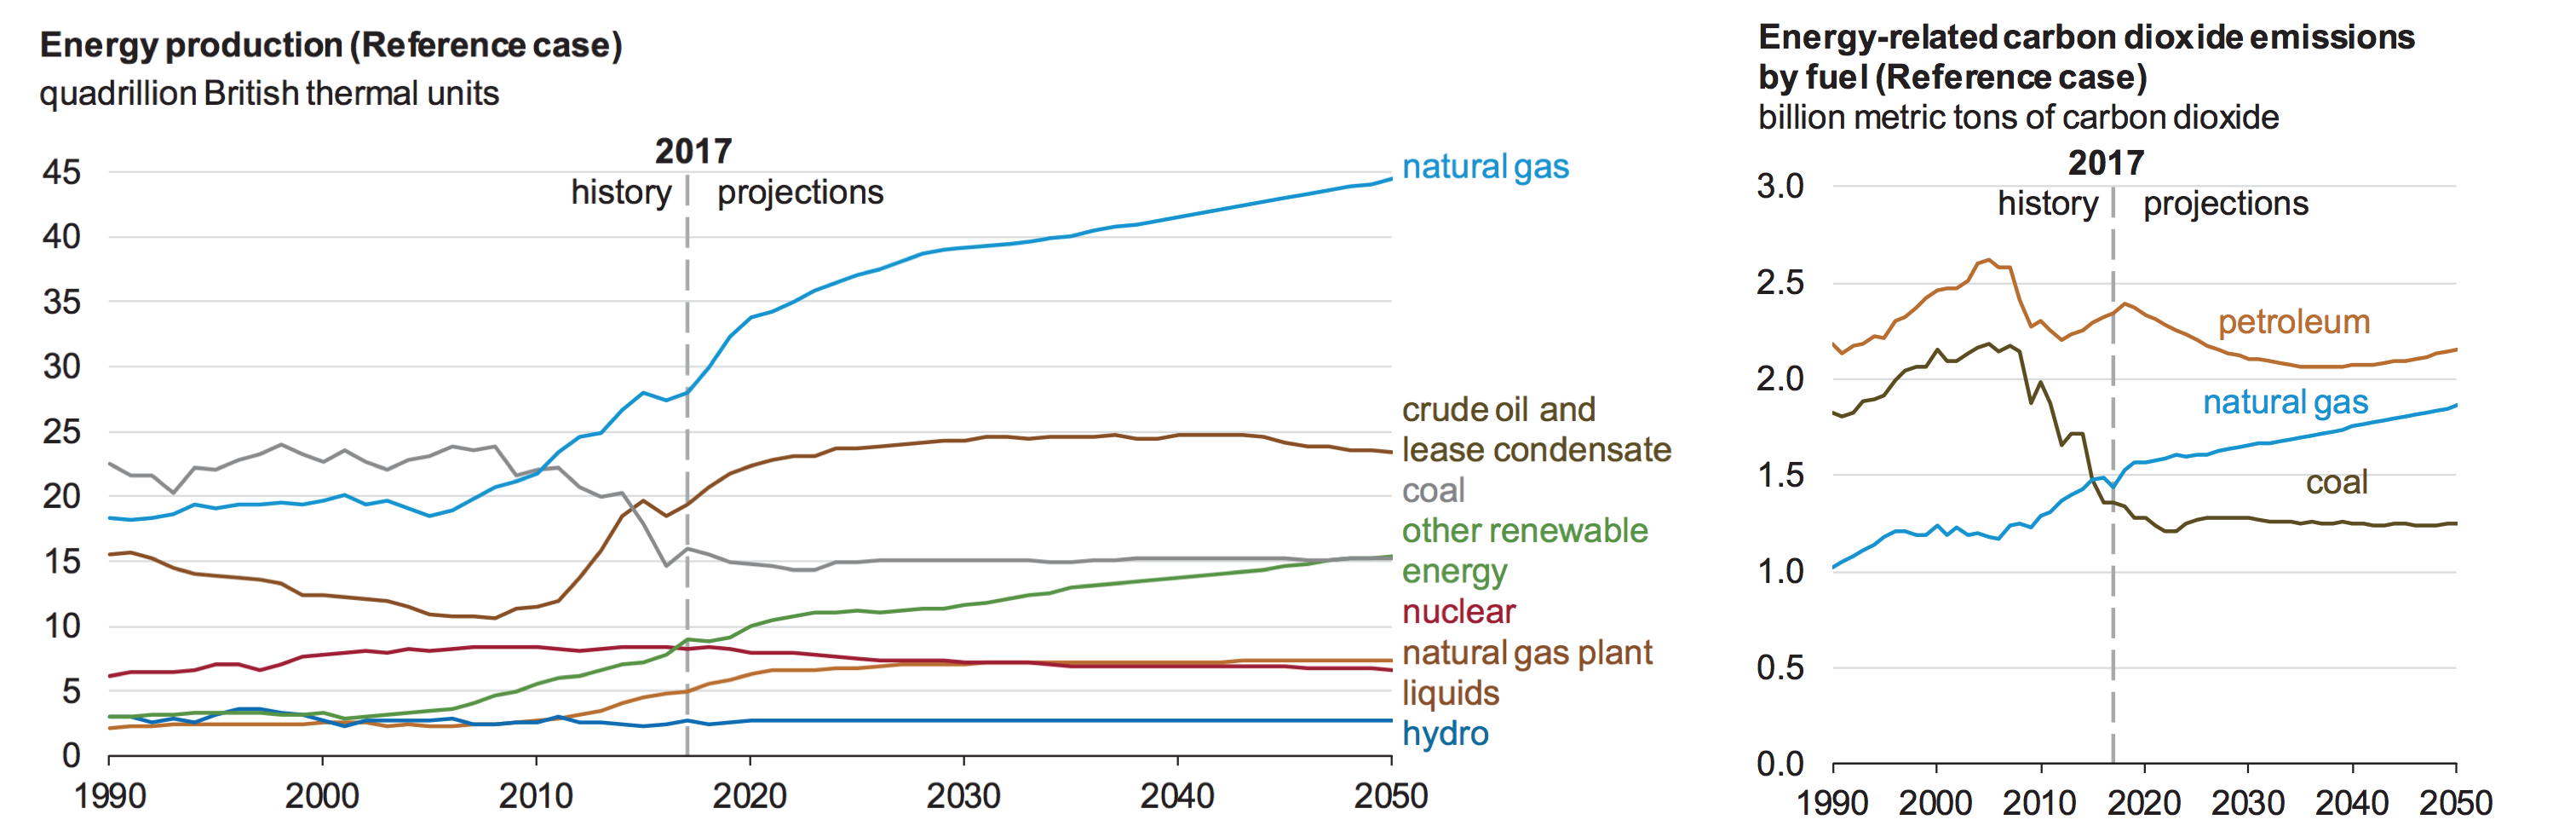
\includegraphics[width=\textwidth]{figures/greenhouse_gas_energy_type.png}	
	\caption{\textbf{Left:} Projected growth of fuel types, based on current trends in the energy market.  \textbf{Right:} Amount of greenhouse gas emissions by energy fuel type, based on projected electricity consumption.  Figures from the Energy Information Administration 2018 Annual Energy Outlook \cite{eia_eo}.}	
\label{fig:ghg}
\end{figure}






